% Created 2020-09-16 Mi 23:10
% Intended LaTeX compiler: pdflatex
\documentclass[a4paper,11pt]{article}
\usepackage[latin1]{inputenc}
\usepackage[T1]{fontenc}
\usepackage{graphicx}
\usepackage{grffile}
\usepackage{longtable}
\usepackage{wrapfig}
\usepackage{rotating}
\usepackage[normalem]{ulem}
\usepackage{amsmath}
\usepackage{textcomp}
\usepackage{amssymb}
\usepackage{capt-of}
\usepackage{hyperref}
\usepackage{pgfplots}
\author{Moaz Haque, Felix Oechelhaeuser, Leo Pirker, Dennis Schulze}
\date{\today}
\title{Analysis I und Lineare Algebra f�r Ingenieurwissenschaften \large  \\ Hausaufgabe 07 - Geuter 29}
\hypersetup{
 pdfauthor={Moaz Haque, Felix Oechelhaeuser, Leo Pirker, Dennis Schulze},
 pdftitle={Analysis I und Lineare Algebra f�r Ingenieurwissenschaften \large  \\ Hausaufgabe 07 - Geuter 29},
 pdfkeywords={},
 pdfsubject={},
 pdfcreator={Emacs 27.1 (Org mode 9.3.6)}, 
 pdflang={English}}
\begin{document}

\maketitle
\tableofcontents

\pagebreak

\section{Aufgabe 1}
\label{sec:org1de58a0}
\subsection{a)}
\label{sec:org1da3fa4}
Es gilt

\begin{align*}
  \frac{1}{b} + \frac{1}{g} &= \frac{1}{f} \\
  \Leftrightarrow \frac{1}{b} &= \frac{g - f}{fg} \\
  \Leftrightarrow b &= \frac{fg}{g - f}
\end{align*}

Damit ist b betrachtet als Funktion

$$ b(g) = \frac{fg}{g - f} $$

\subsection{b)}
\label{sec:org766eec6}
Wenn \(\lim_{n \rightarrow \infty} x_n = a\) und \(x_n \neq a\) gilt, dann gilt

\begin{align*}
    \lim_{n \rightarrow \infty} b(x_n)
    = \frac{\lim_{n \rightarrow \infty}x_n \cdot f}{\lim_{n \rightarrow \infty}x_n-f}
    = \frac{af}{a-f} = b(a)
\end{align*}

daraus folgt \(b(g)\) ist stetig auf \(D(b) = \mathbb{R}\) $\backslash$ \{\(f\)\}.

\subsection{c)}
\label{sec:org2f0c443}
Es gilt f�r den ersten Term

\begin{align*}
  \lim_{g \rightarrow \infty} b(g) &= \lim_{g \rightarrow \infty} \frac{fg}{g - f} \\
  &= \lim_{g \rightarrow \infty} \frac{f}{1 - \frac{f}{g}} \\
  &= \frac{f}{1 - 0} \\
  &= f
\end{align*}

\pagebreak

Es gilt f�r den zweiten Term

\begin{align*}
  \lim_{g \rightarrow f} b(g) &= \lim_{g \rightarrow f} \frac{fg}{g - f} \\
  &= \frac{\lim_{g \rightarrow f} fg}{\lim_{g \rightarrow f} (g - f)} \\
  &= \frac{f^2}{f - f} \\
  &\Rightarrow \lim_{g \rightarrow f} b(g) = \infty
\end{align*}

\section{Aufgabe 2}
\label{sec:org93e1725}
\subsection{a)}
\label{sec:org306a0a9}
Wenn \(\lim_{n \rightarrow \infty}x_n = a\) und \(x_n \neq a\) gelten, \\
dann gilt f�r \(x < 1\)

\begin{align*}
  \lim_{n \rightarrow \infty}(f(x_n))
  &= \lim_{n \rightarrow \infty}(\cos(x_n\pi)+3) \\
  &= \cos(\lim_{n \rightarrow \infty}(x_n)\pi)+3 \\
  &= \cos(a\pi) + 3 = f(a)
\end{align*}

\(\Rightarrow\) \(f\) stetig auf \(\left] -\infty, 1 \right[\) \\

und f�r \(x > 1\)

\begin{align*}
  \lim_{n \rightarrow \infty}(f(x_n))
  &= \lim_{n \rightarrow \infty}(\frac{x_n^2+1}{x_n+1}) \\
  &= \frac{\lim_{n \rightarrow \infty}(x_n)^2+1}{\lim_{n \rightarrow \infty}(x_n)+1} \\
  &= \frac{a^2+1}{a+1} = f(a)
\end{align*}

\(\Rightarrow\) \(f\) stetig auf \(\left] 1, \infty \right[\) \\

Zu �berpr�fen ist noch die Stelle \(x = 1\) \\

Es gilt f�r \(\lim_{x \rightarrow 1^-} f(x)\)

\begin{align*}
  \lim_{x \rightarrow 1^-} f(x) &= \lim_{x \rightarrow 1^-} (\cos(\pi x) + 3) \\
  &= \cos(\pi) + 3 = -1 + 3 = 2
\end{align*}

und es gilt f�r \(\lim_{x \rightarrow 1^+} f(x)\)

\begin{align*}
  \lim_{x \rightarrow 1^+} f(x) &= \lim_{x \rightarrow 1^+} \frac{x^2 + 1}{x + 1} \\
  &= \frac{1^2 + 1}{1 + 1} = \frac{2}{2} = 1
\end{align*}

daraus folgt, dass \(f\) an der Stelle \(x = 1\) nicht stetig ist. \\

Damit ist \(f\) auf \(\mathbb{R}\) $\backslash$ \{1\} stetig.

\subsection{b)}
\label{sec:org487827b}
Der linearaffine Anteil von \(f\) muss die anderen Terme an den jeweiligen Grenzen ber�hren. \\
Daraus ergebt sich

\begin{align*}
  f(-1) &= \frac{1}{-1} = -1 \\
  f(2) &= \ln(2)
\end{align*}

dann die folgenden Punkte P\textsubscript{1}(-1, -1) und P\textsubscript{2}(2, \(\ln(2)\)). \\
Daraus ergeben sich dann folgende Gleichungen

\begin{align*}
  a &= \frac{\ln(2) - (-1)}{2 - (-1)} = \frac{\ln(2) + 1}{3} \\
  b &= f(-1) - a (-1) = \frac{\ln(2) + 1}{3} - 1
\end{align*}

\(f\) ist dann auf \(\mathbb{R}\) stetig, wenn der linearaffine Anteil dem folgenden Term entspricht

$$ \frac{\ln(2) + 1}{3}x + \frac{\ln(2) + 1}{3} - 1 $$

\pagebreak

\section{Aufgabe 3}
\label{sec:org66afb29}
\subsection{a)}
\label{sec:org8d865e1}
Es gelten

\begin{align*}
  f(1) &= 1^6-1-1 = -1 \text{ und} \\
  f(2) &= 2^6-2-1 = 2 \cdot 2 \cdot 2 \cdot 2 \cdot 2 \cdot 2 -2 -1 \\
    &= 64-2-1 = 61
\end{align*}

Da \(f\) stetig ist und \(f(1) < 0\) und \(f(2) > 0\) gelten, muss \(f\) auf
dem Intervall \(\left[1,2\right]\) eine Nullstelle besitzen.

\subsection{b)}
\label{sec:org113b979}
\begin{align*}
  a_0 = 1, \hspace*{3} b_0 = 2 \\
  x_k &= \frac{a+b}{2} \\
  x_0 &= \frac{1+2}{2} = \frac{3}{2} \\
  f\left( \frac{3}{2}\right) &= \frac{3}{2} \cdot \frac{3}{2} \cdot \frac{3}{2} 
  \cdot \frac{3}{2} \cdot \frac{3}{2} \cdot \frac{3}{2} -\frac{3}{2} - 1 \\
  &= \frac{729}{64} -\frac{3}{2} -1 > 0 \\
  \Rightarrow a_1 = 1, \hspace*{3} b_1 = \frac{3}{2} \\
  \vdots
  \\
  a_6 = \frac{9}{8} = 1,125; \hspace*{3} b_6 = \frac{73}{64} = 1,1406
\end{align*}

Das Intervall ist dann [1,125; 1,1406].

\section{Aufgabe 4}
\label{sec:org595eb68}
\subsection{a)}
\label{sec:org0b6c86d}
Es gilt

\begin{align*}
  \frac{f(x) - f(x_0)}{x-x_0} &= \frac{\sqrt{x}-\sqrt{x_0}}{x-x_0} \\
  &= \frac{x-x_0}{(\sqrt{x}+\sqrt{x_0})(x-x_0)} \\
  &= \frac{1}{\sqrt{x}+\sqrt{x_0}}
\end{align*}

damit gilt

\begin{align*}
  \lim_{x \rightarrow x_0} \frac{f(x) - f(x_0)}{x-x_0} &= \lim_{x \rightarrow x_0} \frac{\sqrt{x}-\sqrt{x_0}}{x-x_0} \\
  &= \lim_{x \rightarrow x_0} \frac{1}{\sqrt{x}+\sqrt{x_0}} \\
  &= \frac{1}{2\sqrt{x_0}}
\end{align*}

daraus folgt

$$ \left( \sqrt{x} \right)' = \frac{1}{2\sqrt{x}} $$

\subsection{b)}
\label{sec:org6db50f0}
\subsubsection{(a)}
\label{sec:org1ce9f62}
\begin{align*}
  (5x^3 - 2\sin(3x))' &= (5x^3)' - (2\sin(3x))' \\
    &= 15x^2 - 6\cos(3x)
\end{align*}

\subsubsection{(b)}
\label{sec:orgee2cbfc}
$$ (\cos(x) e^x)' = \cos(x)e^x - \sin(x)e^x $$

\subsubsection{(c)}
\label{sec:org1ef6b74}
$$ (e^{2x^2+11} + 7)' &= e^{2x^2+11} (4x) $$

\subsubsection{(d)}
\label{sec:org2ea4816}
\begin{align*}
  \left( \frac{\sin(x^2 - 2\pi)}{\cos(3\pi - x^2)} \right)' &= 
      \frac{2x\cos(x^2 - 2\pi) \cos(3\pi - x^2) - \sin(x^2 - 2\pi)(-\sin(3\pi - x^2) (-2x))}{\cos^2(3\pi - x^2)} \\
    &= \frac{2x(\cos(x^2 - 2\pi)\cos(3\pi - x^2) - \sin(x^2 - 2\pi)\sin(3\pi - x^2))}{\cos^2(3\pi - x^2)} \\
    &= \frac{2x\cos((x^2 - 2\pi) + (3\pi - x^2))}{\cos^2(3\pi - x^2)} \\
    &= \frac{2x\cos(\pi)}{\cos^2(3\pi - x^2)} \\
    &= \frac{-2x}{\cos^2(\pi - x^2)}
\end{align*}

\section{Aufgabe 5}
\label{sec:org66d5c6a}
F�r die 1. Ableitung von \(f\) gilt

$$ f'(x) = -\frac{2}{(x-2)^2} $$

dann gilt f�r eine beliebige Tangente \(t(x) = ax + b\) am Graphen von \(f\)

\begin{align*}
  a &= f'(x_0) = -\frac{2}{(x_0-2)^2} \\
  b &= f(x_0) - f'(x_0) \cdot x_0 = \frac{2}{x_0-2} + 2 + \frac{2 x_0}{(x_0-2)^2}
\end{align*}

mit der Anforderung, dass \(a = -\frac{1}{2}\) sein muss. Damit gilt

\begin{align*}
  a = -\frac{2}{(x_0-2)^2} &= -\frac{1}{2} \\
  \Leftrightarrow \frac{(x_0-2)^2}{2} &= 2 \\
  \Leftrightarrow (x_0-2)^2 &= 4 \\
  \Leftarrow x_0 - 2 &= \pm 2
\end{align*}

daraus ergeben sich die beiden Stellen \(x_1 = 0\) und \(x_2 = 4\). Daraus folgen dann die beiden Tangenten

\begin{align*}
  t_1(x) &= -\frac{1}{2}x + 1 \\
  t_2(x) &= -\frac{1}{2}x + 5
\end{align*}

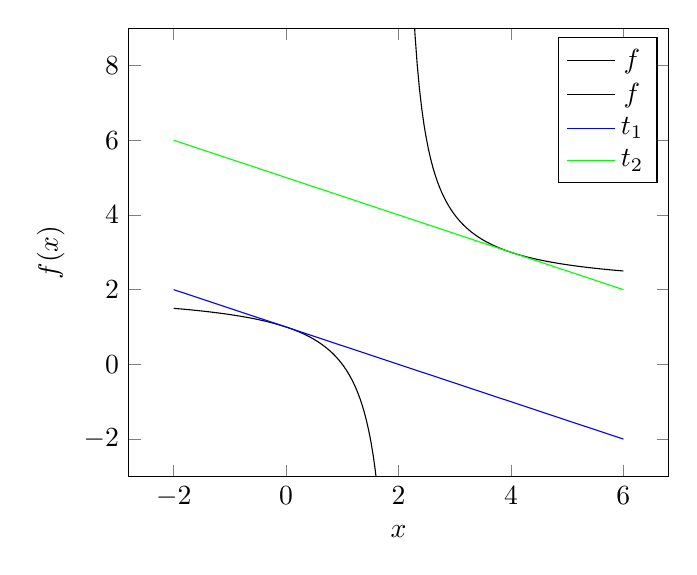
\begin{tikzpicture}
  \begin{axis}[xlabel = $x$, ylabel = {$f(x)$}, ymin=-3, ymax=9]
  \addplot[samples=100, color=black, domain=-2:1.99]{2/(x-2) + 2};
  \addplot[samples=100, color=black, domain=2.01:6]{2/(x-2) + 2};
  \addlegendentry{$f$}
  \addlegendentry{$f$}
  \addplot[color=blue, domain=-2:6]{-1/2 * x + 1};
  \addlegendentry{$t_1$}
  \addplot[color=green, domain=-2:6]{-1/2 * x + 5};
  \addlegendentry{$t_2$}
  \end{axis}
\end{tikzpicture}

\section{Aufgabe 6}
\label{sec:org18ac982}
\subsection{a)}
\label{sec:orgb9d2c74}
\subsection{b)}
\label{sec:org6ce9cb2}
\end{document}